\documentclass[11pt, a4paper]{article}
\usepackage{minted}
\usepackage{multirow}
\usepackage{enumerate}
\usepackage{geometry}
\geometry{left=2.5cm,right=2.5cm,top=2.5cm,bottom=2.5cm}
%\usepackage{minted}
\usepackage[slantfont,boldfont]{xeCJK}
\setCJKmainfont{SimSun}
\usepackage{indentfirst}
\usepackage{float}
\setlength{\parindent}{2em}
\setCJKmonofont{SimHei}
\input zhwinfonts
\renewcommand\figurename{图}
\renewcommand\tablename{表}
\renewcommand\contentsname{\centering 目录}

\begin{document}
\title{{\bf\Huge UpBit的改进} \\[2ex]{\huge 《算法设计与分析》课程第四次作业}}
\author{计算机科学与技术学院\\马玉坤\\1150310618}
\date{2017年6月21日}
\maketitle

\section{对UpBit优化的动机}
\subsection{时间效率}
\subsubsection{对行查询}
\begin{itemize}
\item 更新第k行的值,需要找到第k行修改之前的值。
\item 然而,如图\ref{fig:get_value},寻找第k行的值最坏情况下要遍历所有的位向量。
\item 实际上,作者实验证明,在基数 ({\bf distinct cardinality})等于1000时,get\_value函数耗时占update总耗时的93\%。
\end{itemize}
\begin{figure}[H]
  \begin{center}
    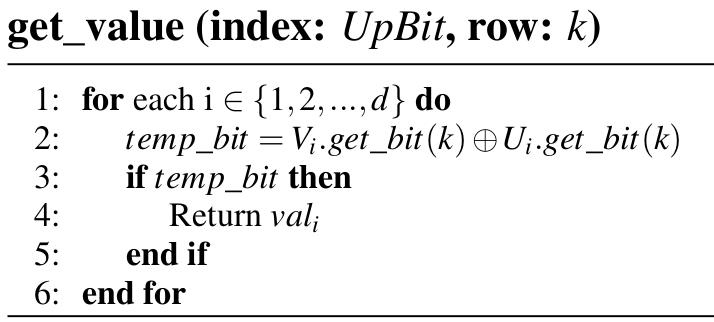
\includegraphics[width=2.8in]{get_value.png}
    \caption{UpBit对行查询}\label{fig:get_value}
  \end{center}
\end{figure}


\subsubsection{范围查询}
  在对数据库查询(例如使用SQL语句)时,我们经常会用到范围查询,比如\\\mintinline{sql}{SELECT * FROM Persons WHERE Year>1965}。

  然而,直接使用UpBit进行范围查询的效率是较低的。最坏情况下需要遍历所有的位向量。

\subsection{空间效率}
\subsubsection{对Update BitVectors的正确认识}
实际上,Update BitVectors在UpBit中起了缓存的作用。而在计算机中,缓存的大小是远远小于主存的大小的。类比计算机系统中的缓存,实际上不需要在内存中为每个位向量都维护一个Update BitVector。甚至可以使用计算机系统中的缓存的替换算法,来有效率地维护Update BitVector。这样做不仅可以减小Update BitVectors内存的占用,还不会降低UpBit的性能。

\section{对UpBit优化的方法}
\subsection{树状数组}
\begin{figure}[H]
  \begin{center}
    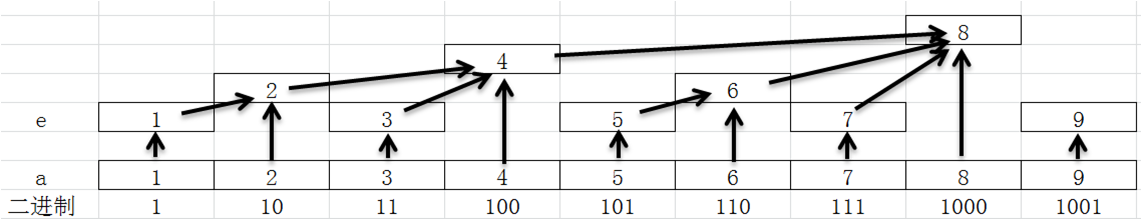
\includegraphics[width=5.0in]{bit.png}
    \caption{树状数组 ({\bf Fenwick Tree})}\label{fig:bit}
  \end{center}
\end{figure}
如图\ref{fig:bit},每个节点对应一个位向量,该位向量为对其子节点的位向量进行或操作后的结果。

每个节点所管辖的区间长度恰好为{\bf 节点编号的二进制表示中最低的1的位置代表的2的幂}。例如6的二进制表示为{\bf 0110},6号节点管辖的区间长度就是2。

\subsection{使用树状数组作为UpBit的组织形式}
\begin{itemize}
\item 对行查询:
  \begin{enumerate}[1.]
  \item 我们要做的是:找到最大的i,使得前i个值的位向量或操作后第k位为0。实际上val[k](第k行的值)即为i+1。
  \item 使用树状数组,我们可以从值的二进制表示中,由最高位到最低位依次确定。
  \item \begin{minted}{C++}
int get_value(int row_id) {
  int col_id = 0;
  for (int i = 0; i <= log2(n); i++) {
    if (ub[col_id+(1<<i)][row_id] ^ vb[col_id+(1<<i)][row_id] == 0) {
      col_id += (1<<i);
    }
  }
  return col_id;
}
  \end{minted}
  \end{enumerate}
\item 范围查询:
  \begin{enumerate}[1.]
  \item 树状数组求前缀和
  \item \begin{minted}{C++}
while (k > 0) {
  res |= val[k];
  k -= lowbit(k);
}
  \end{minted}
  \end{enumerate}
\end{itemize}

\section{实验结果}
\subsection{对行查询效率对比}
\begin{figure}[H]
  \begin{center}
    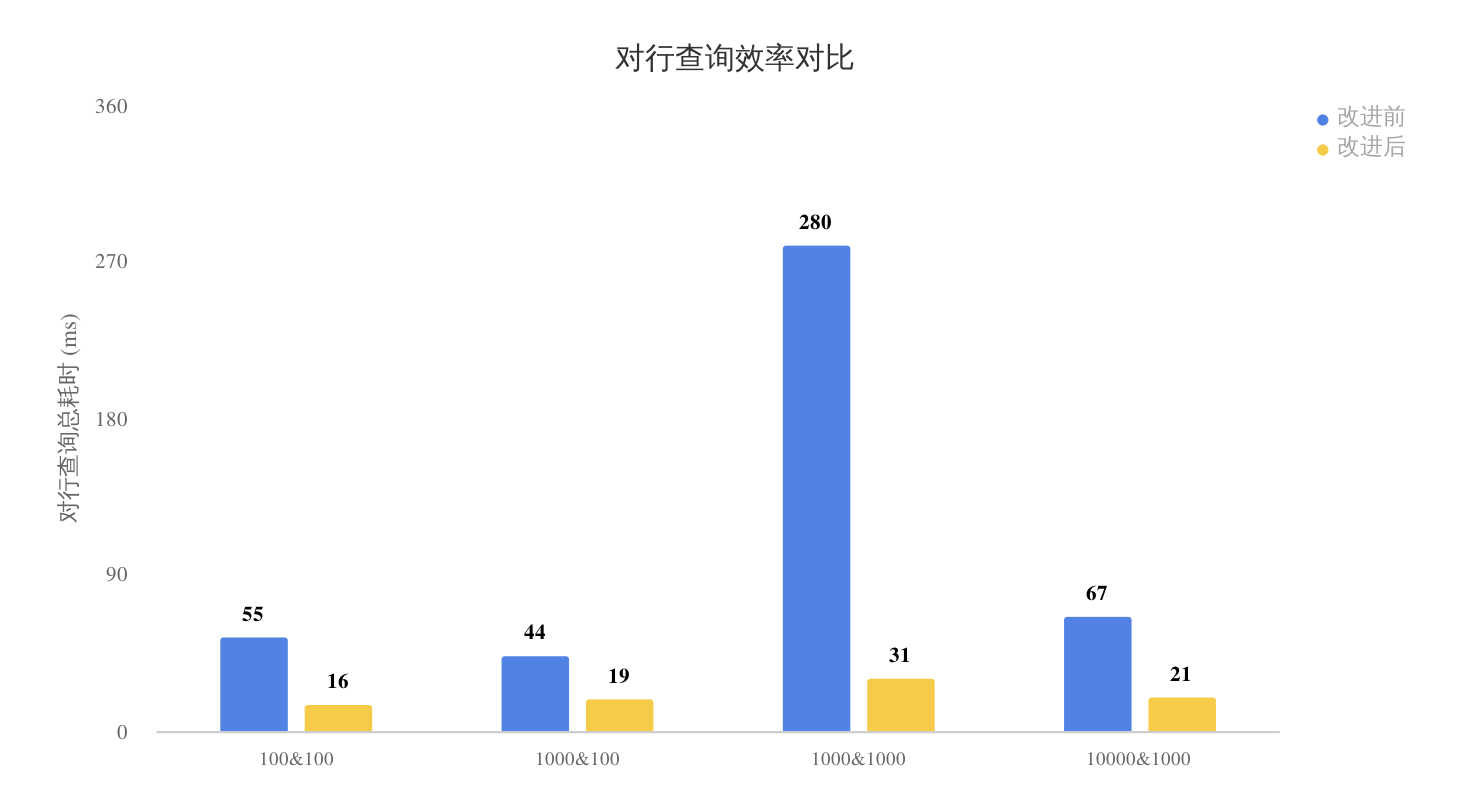
\includegraphics[width=6.5in]{row.png}
    \caption{对行查询效率比较图}\label{fig:row}
  \end{center}
\end{figure}
\subsection{范围查询效率对比}
\begin{figure}[H]
  \begin{center}
    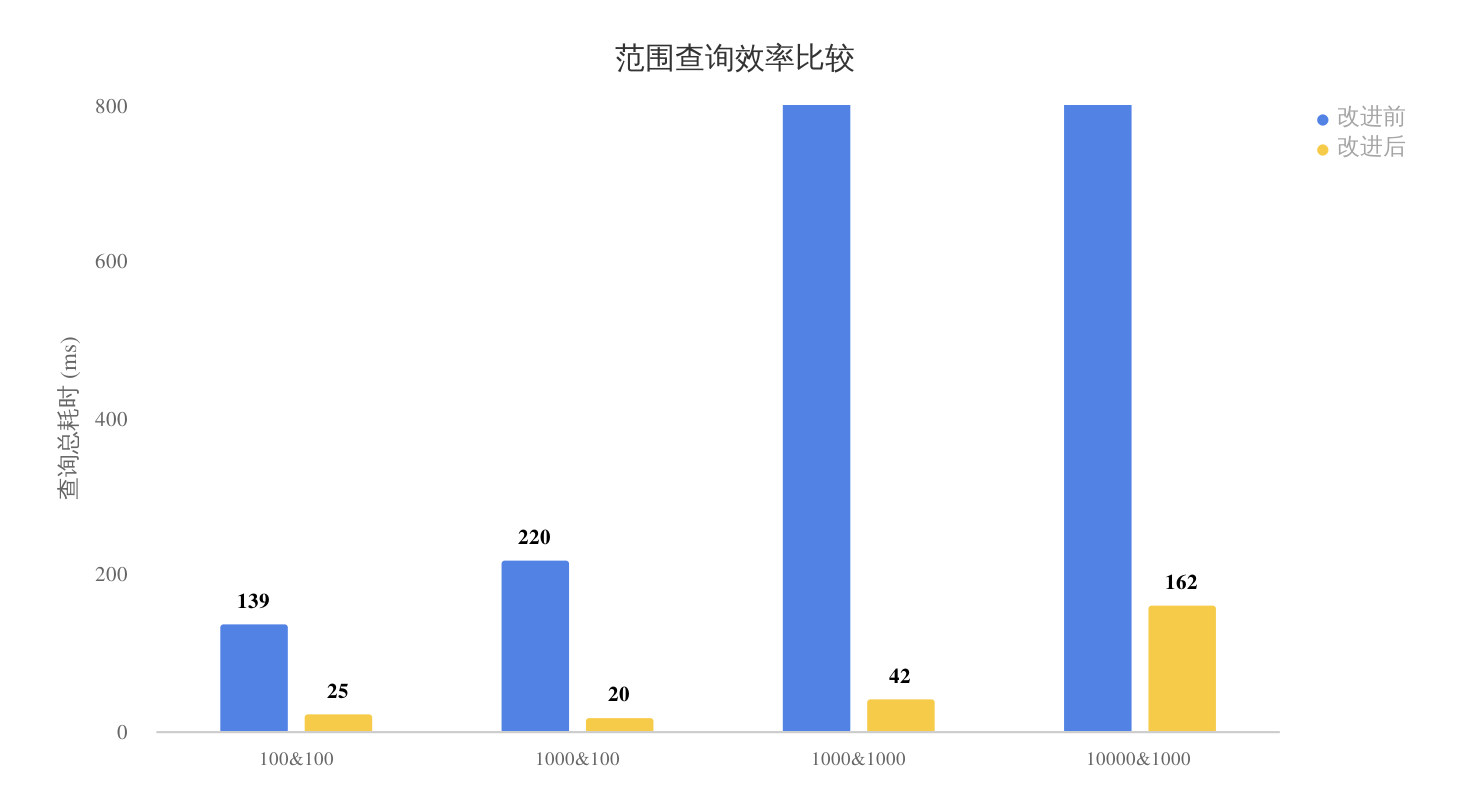
\includegraphics[width=6.5in]{query.png}
    \caption{范围查询效率比较图}\label{fig:query}
  \end{center}
\end{figure}
\subsection{单值修改效率对比}
\begin{figure}[H]
  \begin{center}
    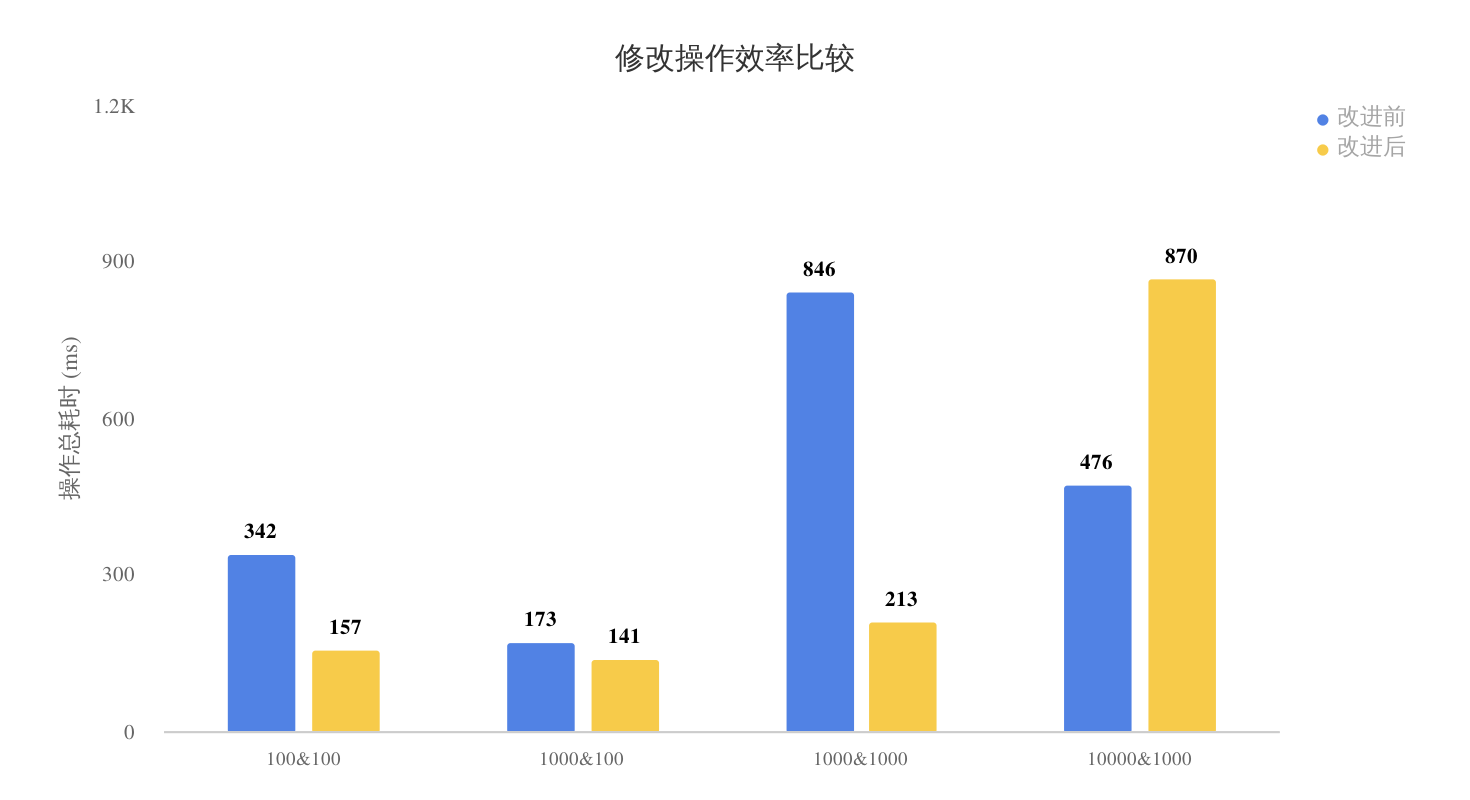
\includegraphics[width=6.5in]{update.png}
    \caption{修改操作效率比较图}\label{fig:update}
  \end{center}
\end{figure}

\section{结论}

\begin{itemize}
\item 改进后的UpBit对于范围查询效率更高
\item 改进后的UpBit在基数较大的情况下修改操作效率更高
\item 改进前的UpBit在基数较小的情况下修改操作效率较高
\item 如果将树状数组修改为其他平衡树(例如Splay),将能够在取值集合未知的情况下,动态向属性的取值集合添加元素。(尽管效率可能下降。)
\item 高效地利用Update BitVector将能在不影响效率的情况下减少其内存使用。
\end{itemize}
\end{document}
